\documentclass{article}

% Course final project (not a conference submission). We use this style file for
% formatting only; [final] shows the author block, and we blank out the conference
% notice/footer below.
\usepackage[final]{neurips_2024}

% Suppress the conference notice printed at the bottom of page 1.
\makeatletter
\renewcommand{\@notice}{}
\makeatother

\usepackage[utf8]{inputenc}   % allow utf-8 input
\usepackage[T1]{fontenc}      % use 8-bit T1 fonts
\usepackage{hyperref}         % hyperlinks
\usepackage{url}              % simple URL typesetting
\usepackage{booktabs}         % professional-quality tables
\usepackage{amsfonts}         % blackboard math symbols
\usepackage{amsmath}
\usepackage{amssymb}
\usepackage{bm}
\usepackage{nicefrac}         % compact symbols for 1/2, etc.
\usepackage{microtype}        % microtypography
\usepackage{xcolor}
\usepackage{graphicx}
\usepackage{algorithm}
\usepackage{algpseudocode}
\usepackage{caption}
\captionsetup{font=small}

\graphicspath{{figures/}}

% ---- notation macros -------------------------------------------------------
\newcommand{\W}{\bm{W}}
\newcommand{\A}{\bm{A}}
\newcommand{\X}{\bm{X}}
\newcommand{\Y}{\bm{Y}}
\newcommand{\E}{\bm{E}}
\newcommand{\Z}{\bm{Z}}
\newcommand{\U}{\bm{U}}
\newcommand{\reals}{\mathbb{R}}
\newcommand{\Wd}{\Delta_{\!W}}
\newcommand{\Ad}{\Delta_{\!A}}
\newcommand{\softthr}{\operatorname{soft}}
\newcommand{\sign}{\operatorname{sign}}
\newcommand{\diag}{\operatorname{diag}}
\newcommand{\tr}{\operatorname{tr}}
\DeclareMathOperator*{\argmin}{arg\,min}

\title{Fused-Regime Student-$t$ Dynamic Bayesian Networks\\
for Cross-Asset Dependency Structure}

\author{%
  John Beecher\thanks{Code and data: \url{https://github.com/0xknxwledge/TTIC31180FinalProject}} \\
  TTIC 31180: Probabilistic Graphical Models \\
  Toyota Technological Institute at Chicago \\
  \texttt{johnsbeecher@gmail.com} \\
}

\begin{document}

\maketitle

\begin{abstract}
We extend DYNOTEARS, a continuous-optimization learner of dynamic Bayesian
networks (DBNs), along two axes motivated by financial time series: a fused
multi-regime penalty, whose scientific object is the sparse \emph{change graph}
$\Wd = \W^{\text{event}}-\W^{\text{ordinary}}$, and a Student-$t$ likelihood for
heavy-tailed residuals. The composite objective combines a smooth heavy-tailed
loss, a nonsmooth sparsity-plus-fusion penalty, and the nonconvex NOTEARS
acyclicity constraint. We solve it with consensus ADMM, applying a closed-form
$K{=}2$ fused-lasso proximal step inside an augmented-Lagrangian outer loop. This
is the directed, regime-conditioned, heavy-tailed analogue of the fused graphical
lasso. On a var-sortability-controlled synthetic benchmark (designs standardized so
var-sortability $=0.50$), the full estimator recovers the change graph $+0.19$ to
$+0.31$ change-$W$ AUROC better than the DYNOTEARS-equivalent across change-edge
count, sample size, and tail heaviness, with the gap widest under heavy tails. The
exact-prox solver is the dominant lever, Student-$t$ and fusion help secondarily,
and held-out-likelihood selection chooses fusion ($\gamma>0$) in every seed. We
then apply the method to a $d=23$ hourly cross-asset panel (2024--2026) around
U.S.\ macro releases (CPI/NFP/FOMC). The contemporaneous DAG is strongly justified
(out-of-sample $\W\equiv 0$ gate: DAG $\gg$ SVAR; Student-$t$ beats Gaussian
density), but the empirical hypothesis is \emph{not} supported: neither the
contemporaneous nor the lagged structure changes around events beyond a
volatility-matched null, at global or edge-wise resolution, and held-out selection
independently drives the fusion penalty $\gamma\to 0$. We report this as a
carefully-controlled negative result, separate from the validated methodological
contribution.
\end{abstract}

\section{Introduction}

DYNOTEARS \citep{pamfil2020dynotears} learns dynamic Bayesian networks (DBNs) from
time series. It assumes a single, stationary series. Its key idea is to recast the
combinatorial search over directed acyclic graphs as continuous optimization, using
the smooth NOTEARS acyclicity surrogate \citep{zheng2018notears}. The estimator is
elegant and widely used. Two settings it handles poorly, however, are exactly the
ones a financial application forces on us. First, heterogeneous regimes: when
calendar information partitions the data into states (e.g.\ ordinary trading versus
a scheduled macroeconomic event) that share most of their dependency structure,
fitting one graph blurs the regimes, while fitting independent graphs wastes the
shared signal, especially when one regime is small. Second, heavy tails: asset
returns have fat tails, so the Gaussian-equivalent squared loss implicit in
DYNOTEARS is a mismatched likelihood that over-weights large innovations.

We propose FR-tDBN (Fused-Regime Student-$t$ DBN), which augments DYNOTEARS with two
ingredients. First, a fused penalty $\gamma\,\|\W^{1}-\W^{0}\|_1$ across $K{=}2$
regimes, so edges that do not change pay no cost and the small event regime borrows
strength from the large ordinary regime; the estimand is the sparse change graph
$\Wd=\W^{1}-\W^{0}$. Second, a fixed-$\nu$ Student-$t$ data term in place of squared
loss. The fused penalty does not produce a sparse $\Wd$ under the smoothed-$\ell_1$
surrogate that NOTEARS-style solvers use, because $\sqrt{x^2+\epsilon}$ never reaches
exactly zero. We therefore solve the true composite objective with consensus ADMM,
applying a closed-form fused-lasso proximal operator (the $K{=}2$ case of
\citealp{friedman2007pathwise,danaher2014jgl}) to the nonsmooth penalties and L-BFGS
to the smooth data-plus-acyclicity part, inside an augmented-Lagrangian loop for the
nonconvex constraint. This is the directed, regime-conditioned, heavy-tailed analogue
of the fused/joint graphical lasso \citep{danaher2014jgl}.

Because real financial graphs have no ground-truth DAG, the methodological claim is
earned on simulation. Our synthetic benchmark explicitly controls for
\emph{var-sortability} \citep{reisach2021varsortability}: the generator is var-sortable
by construction, so we standardize each regime before fitting, pinning measured
var-sortability at $0.50$ and removing the variance gradient that can make NOTEARS-style
methods look good for the wrong reason. On this benchmark FR-tDBN clearly out-recovers
the DYNOTEARS-equivalent, and the win survives a distribution-free rank transform.

We then apply the method to a small but complete $d=23$ crypto--macro panel sampled
hourly over two years, asking a concrete empirical question: \emph{does the
conditional dependency structure linking crypto, equities, rates, FX, and volatility
reorganize around scheduled macro releases (CPI/NFP/FOMC), and which edges flip?}
The contemporaneous DAG is strongly justified. But tested against a
volatility-matched null, the change graph is indistinguishable from chance at both
global and edge-wise resolution, for both contemporaneous and lagged structure.
Principled model selection corroborates this independently by driving the fusion
penalty to zero. We report the null as the defensible empirical statement.

\paragraph{Contributions.}
\begin{enumerate}\itemsep2pt
  \item \textbf{Method.} A fused multi-regime, Student-$t$ DBN whose estimand is a
  sparse change graph, with a consensus-ADMM solver that applies an exact closed-form
  fused-lasso prox inside the NOTEARS augmented-Lagrangian loop (\S\ref{sec:method}).
  \item \textbf{Var-sortability-controlled evidence.} On a standardized benchmark,
  FR-tDBN recovers the change graph $+0.19$ to $+0.31$ AUROC better than the
  DYNOTEARS-equivalent across the design space; we attribute the gain to the
  exact-prox solver (dominant), the Student-$t$ loss, and fusion, via a one-codebase
  ablation, and confirm robustness to a rank transform and to principled $(\lambda,\gamma)$
  selection (\S\ref{sec:synthetic}).
  \item \textbf{A controlled cross-asset null.} On real data we justify the
  contemporaneous DAG out-of-sample, then show with volatility-matched global and
  edge-wise permutation tests (and corroborating held-out selection) that scheduled
  macro events do \emph{not} measurably reorganize the dependency graph at hourly
  resolution (\S\ref{sec:application}).
\end{enumerate}

\section{Method: Fused-Regime Student-$t$ DBN}
\label{sec:method}

\subsection{Model and notation}
Regimes $k\in\{0,1\}$ ($0=$ ordinary, $1=$ event); $d$ variables; lag order $p$;
$n_k$ observations in regime $k$; $N=n_0+n_1$. Per regime the lagged design comprises
contemporaneous targets $\X^k\in\reals^{n_k\times d}$ and lagged copies
$\Y^k_\ell\in\reals^{n_k\times d}$ for $\ell=1,\dots,p$. Parameters
$\Theta=(\W^0,\W^1,\A^0_{1:p},\A^1_{1:p})$ consist of per-regime intra-slice DAGs
$\W^k\in\reals^{d\times d}$ ($\diag(\W^k){=}0$; entry $\W^k[i,j]$ is the directed
edge $i\!\to\!j$, so column $j$ is the structural equation for variable $j$) and
inter-slice matrices $\A^k_\ell$. The residuals are
\begin{equation}
  \E^k \;=\; \X^k - \X^k\W^k - \sum_{\ell=1}^{p}\Y^k_\ell\A^k_\ell
  \qquad (n_k\times d),
\end{equation}
modeled i.i.d.\ Student-$t$ with shared, fixed degrees of freedom $\nu$ and fixed
per-variable scales $\sigma_j$ (pooled robust MAD).

\subsection{Objective}
We minimize $F(\Theta)=f(\Theta)+g(\Theta)$ subject to per-regime acyclicity. The
smooth data term is normalized per observation so penalties transfer across
$n$ (the larger ordinary regime carries proportionally more weight, which is the
borrow-strength mechanism):
\begin{equation}
  f(\Theta) \;=\; \frac{1}{N}\sum_{k\in\{0,1\}}\sum_{t=1}^{n_k}\sum_{j=1}^{d}
  \ell\!\left(\E^k[t,j];\,\nu,\sigma_j\right),
\end{equation}
with, at fixed $\nu,\sigma$ (additive $\nu$-constants dropped for training; restored
for held-out density, \S\ref{sec:eval}),
\begin{equation}
  \ell_{t}(e;\nu,\sigma)=\log\sigma+\tfrac{\nu+1}{2}\log\!\Big(1+\tfrac{e^2}{\nu\sigma^2}\Big),
  \qquad
  \ell_{\mathcal N}(e;\sigma)=\log\sigma+\tfrac{e^2}{2\sigma^2}.
\end{equation}
The nonsmooth penalty combines within-regime sparsity and cross-regime fusion,
\begin{equation}
\begin{aligned}
  g(\Theta)=\;&\lambda_W\big(\|\W^0\|_1+\|\W^1\|_1\big)
  +\lambda_A\!\sum_\ell\big(\|\A^0_\ell\|_1+\|\A^1_\ell\|_1\big)\\
  &+\underbrace{\gamma_W\|\W^1-\W^0\|_1}_{\text{fusion}}
  +\gamma_A\!\sum_\ell\|\A^1_\ell-\A^0_\ell\|_1,
\end{aligned}
\end{equation}
subject to $h(\W^k)=0$ and $\diag(\W^k)=0$, where $h(\W)=\tr\!\big(e^{\W\circ\W}\big)-d$
is the NOTEARS surrogate ($\circ$ = Hadamard product). Here $f$ is smooth, $g$ is
convex but nonsmooth, and $h$ is smooth but nonconvex; the fusion term is the heart of
the model, since unchanged edges pay no cost and the reported object is the sparse
$\Wd=\W^1-\W^0$.

\subsection{Optimization}
\label{sec:opt}
We separate the three term types: L-BFGS for the smooth part, an
augmented-Lagrangian outer loop for the nonconvex acyclicity, and a closed-form
proximal operator for the nonsmooth penalties via consensus ADMM
\citep{boyd2011admm}. The idea of ADMM is to give the smooth and the nonsmooth terms
their own copy of the parameters, let each subproblem solve the piece it is suited to
(gradients for the smooth loss, thresholding for the penalties), then reconcile the
copies. Concretely, introduce penalty copies
$\Z=(\bm V^0,\bm V^1,\bm B^0_{1:p},\bm B^1_{1:p})$ of $\Theta$ under the consensus
constraint $\Theta=\Z$, together with a scaled dual variable $\U$ that accumulates the
running disagreement $\Theta-\Z$ and is what forces the two copies to exact equality at
a finite penalty $\rho$. The smooth subproblem the L-BFGS step sees is
\begin{equation}
  S(\Theta)=f(\Theta)+\sum_k\Big[\tfrac{\rho_h}{2}h(\W^k)^2+\alpha_k\,h(\W^k)\Big].
\end{equation}

\begin{algorithm}[t]
\caption{FR-tDBN: consensus ADMM inside the acyclicity augmented Lagrangian}
\label{alg:admm}
\begin{algorithmic}[1]
\State \textbf{init} $\Theta\sim$ small random ($\diag\W{=}0$); $\Z\!\gets\!\Theta$;
       $\U\!\gets\!0$; $\alpha\!\gets\!0$; $\rho_h\!\gets\!1$; $h_{\text{prev}}\!\gets\!\infty$
\For{outer $m=1,\dots,M$} \Comment{acyclicity augmented Lagrangian}
  \For{$t=1,\dots,T_{\text{admm}}$} \Comment{consensus ADMM}
    \State $\Theta \gets \argmin_\Theta\; S(\Theta)+\tfrac{\rho}{2}\|\Theta-\Z+\U\|_F^2$
           \Comment{smooth: L-BFGS, strong-Wolfe}
    \State $\Z \gets \textsc{FusedProx2}\big(\Theta+\U;\ \lambda/\rho,\ \gamma/\rho\big)$
           \Comment{closed-form, exact zeros; $\diag\bm V{=}0$}
    \State $\U \gets \U + \Theta - \Z$ \Comment{dual update}
  \EndFor
  \State $h_{\max}\gets\max_k|h(\W^k_\Theta)|$
  \If{$h_{\max}>0.25\,h_{\text{prev}}$ \textbf{and} $\rho_h<\rho_h^{\max}$}
       \State $\rho_h\gets 10\,\rho_h$
  \Else\ \State $\alpha_k\gets\alpha_k+\rho_h\,h(\W^k_\Theta)$;\quad $h_{\text{prev}}\gets h_{\max}$
  \EndIf
  \State \textbf{if} $h_{\max}\le h_{\text{tol}}$ \textbf{break}
\EndFor
\State \textbf{report} $\W^k\!\gets\!\bm V^k$ (exactly sparse), $\A^k_\ell\!\gets\!\bm B^k_\ell$,
       $\Wd=\bm V^1-\bm V^0$, $\Ad=\bm B^1-\bm B^0$
\end{algorithmic}
\end{algorithm}

The $\Theta$-update is smooth (the only nonconvexity is $h^2$), so L-BFGS is
well-behaved; all sparsity and fusion live in the $\Z$-update. A proximal operator
$\operatorname{prox}_{h}(a)=\argmin_v h(v)+\tfrac12\|v-a\|^2$ returns the point that
lowers a penalty $h$ while staying near its input $a$; for an $\ell_1$ penalty it is
soft-thresholding, which shrinks each coordinate toward zero and snaps small ones to
\emph{exactly} zero (the source of sparsity). Our $K{=}2$ fused-lasso prox
\citep{tibshirani2005fused,friedman2007pathwise} applies two such pulls at once: each
weight is pulled small ($\ell_1$) and the two regimes are pulled equal (fusion). For
each coordinate, $\textsc{FusedProx2}(a^0,a^1;\lambda',\gamma')$ solves
$\min_{v}\ \tfrac12(v^0{-}a^0)^2+\tfrac12(v^1{-}a^1)^2+\lambda'(|v^0|{+}|v^1|)+\gamma'|v^1{-}v^0|$
by \emph{fuse, then soft-threshold}. The fuse step (preserving the mean $(a^0{+}a^1)/2$) is
\begin{equation}
(t^0,t^1)=
\begin{cases}
(a^0+\gamma',\ a^1-\gamma') & \text{if } a^1-a^0>2\gamma'\\
(a^0-\gamma',\ a^1+\gamma') & \text{if } a^1-a^0<-2\gamma'\\
\big((a^0{+}a^1)/2,\ (a^0{+}a^1)/2\big) & \text{otherwise,}
\end{cases}
\end{equation}
followed by the soft-threshold $v^k=\sign(t^k)\max(|t^k|-\lambda',0)$.
The difference is soft-thresholded by $2\gamma'$, forcing $\W^0=\W^1$ (hence exact
zeros in $\Wd$) on unchanged edges, which is the selection behavior smoothed-$\ell_1$ lacks.
Empirically $\max_k h(\W^k)\approx 4\times10^{-3}$ at convergence, and ADMM $\times$
nonconvex acyclicity did not require the warm-start fallback we had budgeted for.

\subsection{Variants and ablations}
A single codebase exposes four orthogonal switches, enabling fair attribution. The
loss $\in\{\text{Student-}t,\text{Gaussian}\}$ isolates heavy tails; the fusion
strength toggles $\gamma{=}0$ (independent per-regime fits) against $\gamma{>}0$; the
solver $\in\{\texttt{admm}$ (exact prox, headline), $\texttt{lbfgs\_smooth}$ (smoothed
$\sqrt{x^2+\epsilon}$, the DYNOTEARS-style baseline)$\}$ isolates the prox; and an
adaptive-fusion option sets $\gamma_{ij}=\gamma_0/(|\hat\Delta_{ij}|+\epsilon)$.
The Gaussian, independent, smoothed-$\ell_1$ corner is our reimplementation of
DYNOTEARS, labeled the ``DYNOTEARS-equivalent'' throughout.

\section{Synthetic benchmark}
\label{sec:synthetic}

\paragraph{Generator and var-sortability control.}
\texttt{make\_regime\_pair} samples an Erd\H{o}s--R\'enyi ordinary DAG, stabilizes the
reduced-form VAR, then applies a single stable step to a sparse delta
(additions, removals, reweights), so the change masks equal the realized $\W^1-\W^0$
and $\A^1-\A^0$ exactly (no rescale contamination), $\Wd$ stays sparse, and regime
sizes can be imbalanced ($n_{\text{event}}\ll n_{\text{ordinary}}$). The generator is
var-sortable by construction (variance grows down the topological order; raw score
$\approx 0.83$ at $\nu{=}5$), so we \emph{standardize each regime} before fitting.
This pins measured var-sortability at exactly $0.50$
\citep{reisach2021varsortability}, so recovery cannot ride the variance gradient and the
result transfers to the standardized real pipeline. We score change-edge AUROC, the
ranking of $|\widehat{\Wd}_{ij}|$ against the true change support.

\paragraph{Headline grid.}
Table~\ref{tab:grid} reports change-$W$ AUROC over a solver $\times$ loss $\times$
fusion grid, $24$ fits per cell. Three findings are robust at $\gtrsim 2$ s.e.\ in
both the balanced/moderate-tail regime ($\nu{=}5$, $n\in\{50,100\}$) and the
small-sample/heavy-tail regime ($\nu{=}3$, $n\in\{20,35\}$):
(i) the exact-prox ADMM solver \emph{dominates} smoothed-$\ell_1$ everywhere
($+0.13$ or more), and even ADMM-independent beats smooth-fused, so the solver is the
single largest lever; (ii) Student-$t$ helps under ADMM ($+0.10$ to $0.12$ over
Gaussian); and (iii) fusion helps the weaker (Gaussian) estimator
($+0.06$ to $0.08$) and the balanced regime, while its marginal gain on top of
Student-$t$ is within noise. The full FR-tDBN (ADMM, Student-$t$, fused) is the
best or statistically-tied-best cell in both regimes.

\begin{table}[t]
\centering
\small
\begin{tabular}{llcccc}
\toprule
& & \multicolumn{2}{c}{$\nu=5$,\ \ $n\in\{50,100\}$} & \multicolumn{2}{c}{$\nu=3$,\ \ $n\in\{20,35\}$}\\
\cmidrule(lr){3-4}\cmidrule(lr){5-6}
solver & loss & independent & fused & independent & fused\\
\midrule
\texttt{admm}         & Gaussian   & 0.714 (.030) & 0.794 (.032) & 0.565 (.033) & 0.626 (.027)\\
\texttt{admm}         & Student-$t$ & 0.838 (.027) & \textbf{0.853 (.031)} & \textbf{0.666 (.033)} & 0.662 (.027)\\
\texttt{lbfgs\_smooth}& Gaussian   & 0.584 (.033) & 0.582 (.033) & 0.538 (.031) & 0.562 (.032)\\
\texttt{lbfgs\_smooth}& Student-$t$ & 0.617 (.033) & 0.626 (.031) & 0.524 (.029) & 0.537 (.032)\\
\bottomrule
\end{tabular}
\caption{Synthetic change-$W$ AUROC, mean (s.e.) over $24$ fits/cell, designs
standardized so var-sortability $=0.50$. Best per block in \textbf{bold}.}
\label{tab:grid}
\end{table}

\paragraph{Sweeps across the design space.}
Figure~\ref{fig:sweep} sweeps one axis at a time ($12$ seeds), comparing the full
FR-tDBN against the DYNOTEARS-equivalent. The gap is large and stable: change-edge
count $1{\to}5$, $+0.25$ to $+0.30$; sample size $50{\to}200$, $+0.27$ to $+0.30$;
and tail heaviness $\nu\,3{\to}30$, $+0.31$ (heavy) down to $+0.19$ ($\approx$ Gaussian).
The gap is \emph{largest under heavy tails}, exactly as the Student-$t$ likelihood predicts.
A change-edges-$=0$ control gives a clean $\Wd$-floor ($\|\widehat{\Wd}\|_1\approx 0.27$),
confirming the estimator does not hallucinate change where there is none.

\begin{figure}[t]
\centering
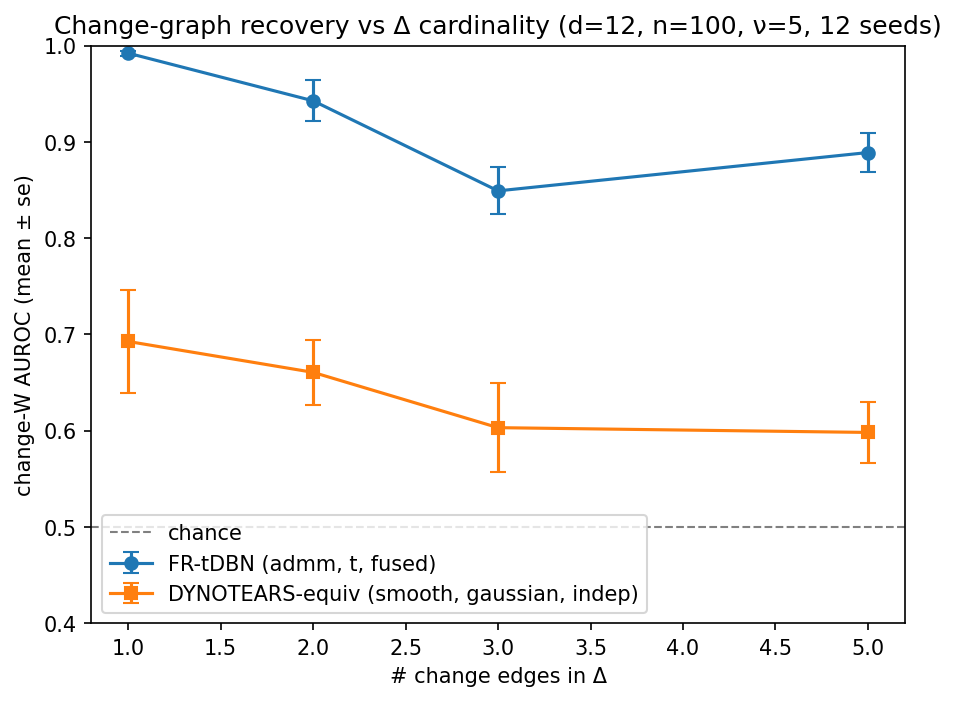
\includegraphics[width=0.66\textwidth]{synthetic_sweep_change_edges.png}
\caption{Change-graph recovery vs.\ $\Wd$ cardinality ($d{=}12$, $n{=}100$, $\nu{=}5$,
$12$ seeds). FR-tDBN (ADMM, Student-$t$, fused) recovers the change support far above
the DYNOTEARS-equivalent (smoothed-$\ell_1$, Gaussian, independent) across the sweep;
both stay above chance ($0.5$). The advantage is reproduced over sample-size and
tail-heaviness sweeps (text).}
\label{fig:sweep}
\end{figure}

\paragraph{Robustness of the methodological claim.}
Two checks guard against artifacts. \emph{(a) Rank transform.} Replacing
standardization with a distribution-free rank (Gaussian-copula) transform shrinks the
FR-tDBN advantage from $+0.24$ to $+0.14$ change-$W$ AUROC but leaves it clearly
positive. The shrinkage is expected, since ranking compresses the heavy tails the
Student-$t$ exploits, so the win is not a marginal-distribution artifact.
\emph{(b) Principled $(\lambda,\gamma)$ selection.} Selecting penalties by held-out
NLL on ground-truth data chooses fusion ($\gamma{=}0.02>0$) in $5/5$ seeds (modal
$\lambda{=}0.03$); BIC is more conservative ($\lambda{=}0.1$, small $\gamma$). Fusion
is thus chosen by a predictive criterion, not hand-tuned. We note that the
held-out $\lambda$ sits at the grid's low edge while BIC's sits high, so the scientific
parameter $\gamma$ is the stable, interpretable one.

\paragraph{A documented negative ablation.}
Adaptive fusion ($\gamma_{ij}=\gamma_0/(|\hat\Delta_{ij}|+\epsilon)$, in the spirit of
\citealp{zou2006adaptive,candes2008reweighted}) \emph{fails} here: at small event-$n$
every available pilot already shrinks the true $\Delta$, so the reweighting
over-penalizes the genuine change edges and collapses $\Wd$ to near-empty. The
unbiased-pilot assumption is violated; we report the failure rather than omit it.
A related limitation is that exact support recovery (F1) at small event-$n$ is
hard even for uniform fusion (F1$\approx 0.22$), which is why we report AUROC and adopt
stability selection on real data rather than trusting a single fit's support.

\section{Cross-Asset Structure Around U.S. Macroeconomic Releases}
\label{sec:application}

We now ask whether the conditional dependency structure linking equities, rates, FX,
commodities, volatility, and crypto reorganizes around scheduled U.S.\ macro releases
(CPI/NFP/FOMC). The panel is deliberately cross-asset: crypto is one block among six.
We give the crypto names modest extra attention because their returns are the most
heavily tailed in the panel, which is exactly where the Student-$t$ likelihood earns
its keep, but the question and the panel are macro-wide rather than crypto-specific.

\subsection{Data and event regime}
We use hourly close prices from Yahoo Finance over the common window
2024-05-30 to 2026-05-28 (UTC), giving $2{,}962$ hourly bars across $499$ trading days
with zero missing returns after alignment to the common trading grid. The $d=23$ panel
spans six blocks (Table~\ref{tab:panel}). Construction floors each timestamp to the
hour, aligns on the union grid, takes log returns, drops any-NaN rows, then applies a
rolling past-only $z$-score (window $250$, min-periods $60$; no look-ahead)
before building the lagged design. We use $p=1$, justified empirically below.

\begin{table}[t]
\centering
\small
\begin{tabular}{ll}
\toprule
block & members\\
\midrule
equity / crypto-equity & SPY, QQQ, IWM, NVDA, COIN, MSTR\\
rates / credit         & TLT, IEF, SHY, HYG\\
commodities            & GLD, SLV, USO\\
FX                     & DXY, EURUSD, GBPUSD, JPY\\
volatility             & VIX\\
crypto (spot)          & BTC, ETH, SOL, XRP, LINK\\
\bottomrule
\end{tabular}
\caption{The $d=23$ cross-asset panel; crypto is one of the six blocks.}
\label{tab:panel}
\end{table}

The event regime comes from \texttt{data/events.csv}, which holds CPI/NFP/FOMC release
times (08:30 ET for CPI/NFP, 14:00 ET for FOMC), verified against official BLS/Fed
schedules including the 2025 lapse-driven exceptions, converted ET$\to$UTC with DST
awareness. Bars within $\pm2$h of a release are tagged event, giving $104$ event bars
(3.6\%): the small-$n_{\text{event}}$ borrow-strength regime the fusion targets. Because
08:30-ET CPI/NFP precede the cash-equity open, their windows on this RTH panel capture
the post-open reaction; FOMC at 14:00 ET is mid-session and captured directly.

\subsection{Evaluation protocol}
\label{sec:eval}
With no ground-truth DAG on real data, we rely on out-of-sample density and controlled
nulls. We use a time-ordered train/test split (last $20\%$ held out) with
train-derived scales for every held-out number (no leakage), and a full-density
NLL (restoring the $\Gamma$ and $\tfrac12\log(\nu\pi)$ constants) so that
Student-$t$-vs-Gaussian and DAG-vs-($\W\!\equiv\!0$) comparisons are valid. The
$\W\!\equiv\!0$ SVAR ablation is the acyclicity/frequency sanity check: only an
out-of-sample win counts, since the DAG has strictly more parameters. We assess
change edges by block-bootstrap stability selection
\citep{meinshausen2010stability} and test significance with global and
edge-wise permutation nulls on both $\Wd$ and $\Ad$ that are block- and
volatility-matched (event windows are mechanically high-volatility), with
Benjamini--Hochberg FDR control \citep{benjamini1995fdr} on the edge-wise tests.

\subsection{Results}

\paragraph{The contemporaneous DAG is real (OOS $\W\!\equiv\!0$ gate).}
Table~\ref{tab:oos} shows every DAG model beats the $\W\!\equiv\!0$ SVAR
out-of-sample by a wide margin (roughly $4.4$k nats for Student-$t$ and $7$k
nats for Gaussian), so the hourly contemporaneous structure genuinely carries the
dependency information. Student-$t$ density beats Gaussian for every model, confirming
heavy tails on real data. This also reads as explanatory power of the joint structure,
not forecasting.

\paragraph{Recovery wins, held-out density does not (vs.\ DYNOTEARS).}
The same table draws the key distinction. On ground-truth \emph{recovery} FR-tDBN beats
the DYNOTEARS-equivalent (\S\ref{sec:synthetic}), but on real-data held-out density it
does not: pooled Gaussian DYNOTEARS is slightly better (roughly $160$ to $360$ nats),
because the thin event regime gives fusion little to exploit out of sample. The
defensible claim is better change-graph recovery on ground truth, not better held-out
density on this panel.

\begin{table}[t]
\centering
\small
\begin{tabular}{lcc}
\toprule
model & Student-$t$ NLL & Gaussian NLL\\
\midrule
FR-tDBN (\texttt{admm}, Student-$t$, fused)        & 13{,}839 & 14{,}738\\
DYNOTEARS-per-regime (smooth, Gaussian, indep)     & 13{,}676 & 14{,}456\\
DYNOTEARS-pooled (smooth, Gaussian, single graph)  & \textbf{13{,}637} & \textbf{14{,}381}\\
SVAR ($\W\equiv 0$)                                & 18{,}287 & 21{,}573\\
\bottomrule
\end{tabular}
\caption{Out-of-sample test NLL (nats; lower is better) on the held-out final $20\%$.
DAG models crush the $\W\!\equiv\!0$ SVAR; Student-$t$ beats Gaussian throughout;
among DAGs, pooled DYNOTEARS edges FR-tDBN on held-out density (the recovery
advantage is on synthetic ground truth, Table~\ref{tab:grid}). Best in \textbf{bold}.}
\label{tab:oos}
\end{table}

\paragraph{Stable change edges are on-thesis but not event-specific.}
Across $25$ block bootstraps the most stable $\Wd$ edges (frequency $1.0$) are
crypto-internal and cross-asset: ETH$\leftrightarrow$SOL/LINK/XRP, BTC$\leftrightarrow$XRP,
BTC$\to$VIX, NVDA$\to$COIN, MSTR$\to$SPY/QQQ, DXY$\to$JPY (Fig.~\ref{fig:heatmaps}, right
panel). The crypto block reliably reorganizes across bootstraps, but, as the nulls
below show, this is sampling-stability, not event-specificity.

\begin{figure}[t]
\centering
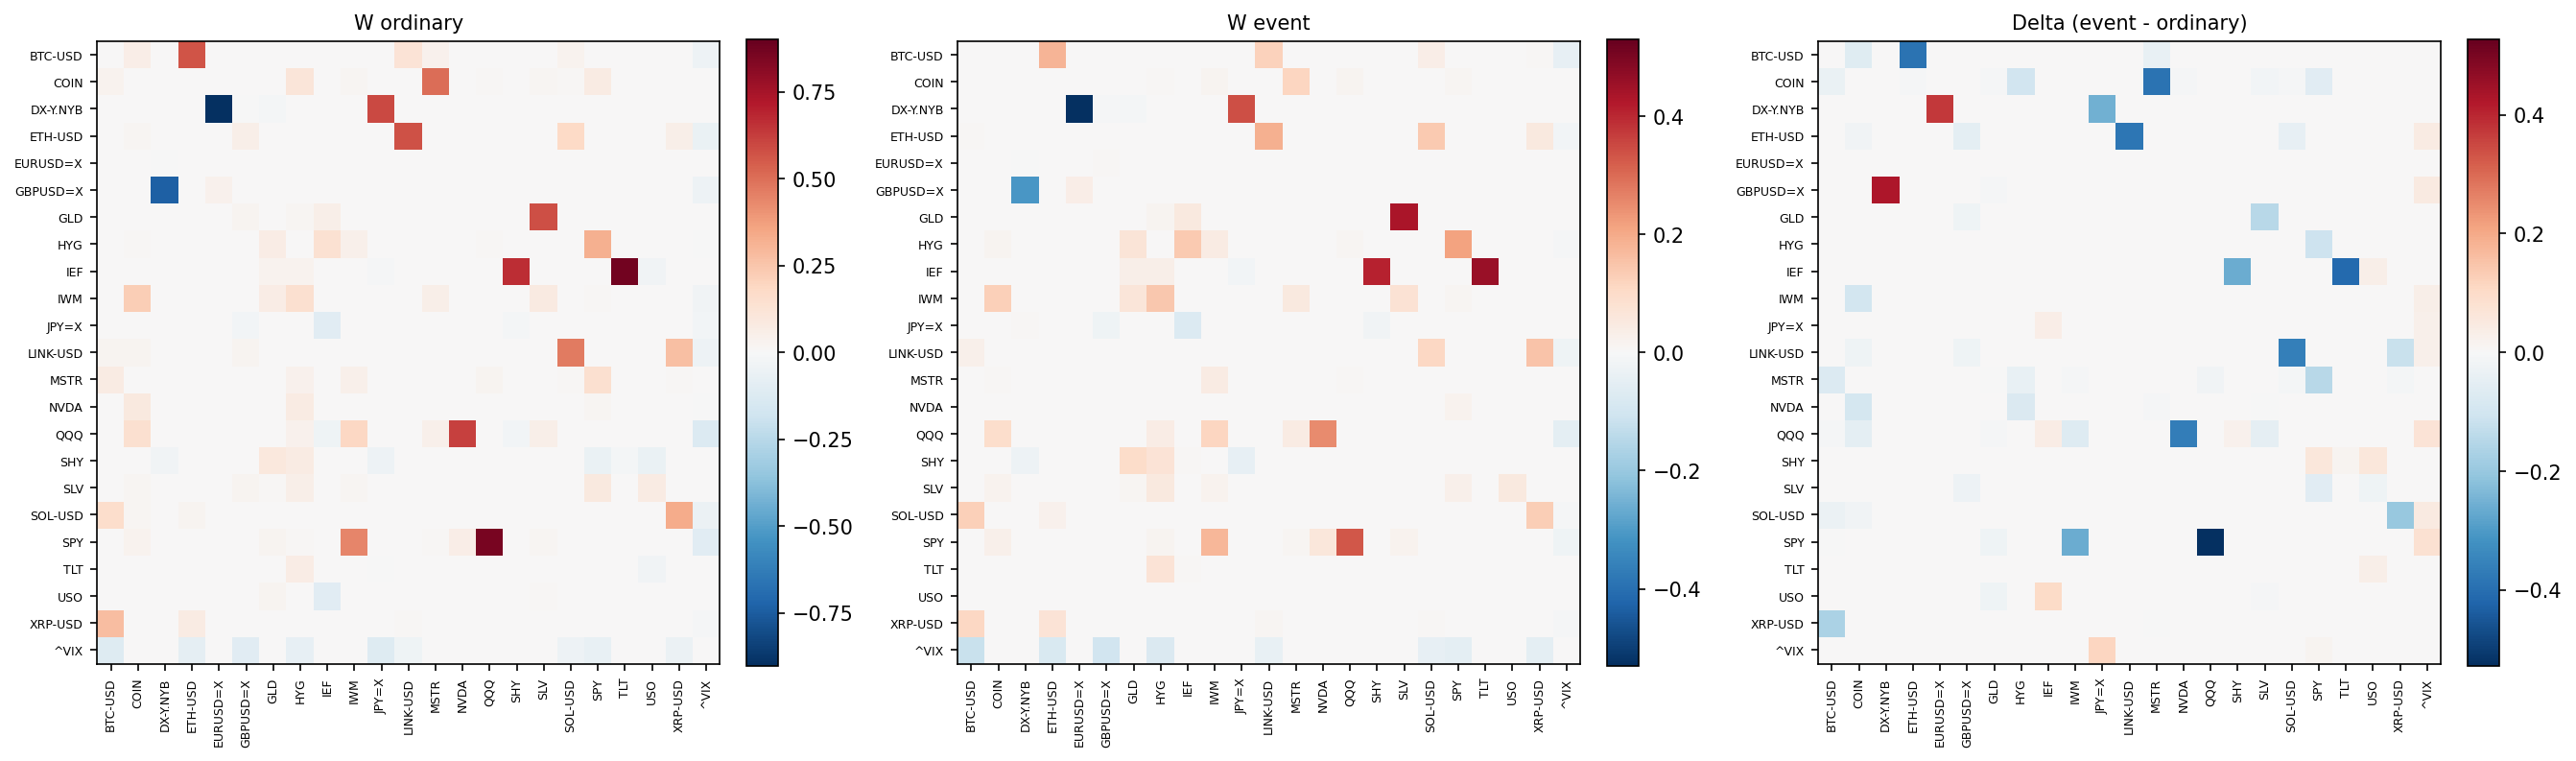
\includegraphics[width=\textwidth]{regime_heatmaps.png}
\caption{Estimated contemporaneous structure on the real panel: ordinary $\W^0$ (left),
event $\W^1$ (middle), and the change graph $\Wd=\W^1-\W^0$ (right). The two regimes
share most structure; the fused estimator concentrates differences into a sparse $\Wd$.
The global magnitude of $\Wd$, however, is not beyond a volatility-matched null
(Table~\ref{tab:nulls}).}
\label{fig:heatmaps}
\end{figure}

\paragraph{The change graph is null (global and edge-wise).}
This is the central empirical result. \emph{Globally}, observed $\|\Wd\|_1=8.10$
against a volatility/block-matched regime-label null with mean $8.91$ ($p\approx 0.81$):
the magnitude of change is not beyond random vol-matched relabeling.
\emph{Edge-wise}, only $10$ edges reach raw $p<0.05$ versus $\approx 25$ expected by
chance, and $0$ survive BH-FDR. The change is concentrated neither in
magnitude nor in specific edges. The result is robust across event type and window
(Table~\ref{tab:nulls}): every observed $\|\Wd\|_1$ is at or below its matched-null
mean (all $p\ge 0.52$).

\begin{table}[t]
\centering
\small
\begin{tabular}{lcccc}
\toprule
setting & $n_{\text{event}}$ & observed $\|\Wd\|_1$ & null mean & $p$\\
\midrule
type = FOMC   & 60  & 11.80 & 13.37 & 1.00\\
type = CPI    & 22  & 14.64 & 14.66 & 0.76\\
type = NFP    & 22  & 14.55 & 14.64 & 0.95\\
window $\pm$1h & 45  & 12.26 & 14.17 & 1.00\\
window $\pm$2h & 104 & \phantom{0}8.10 & \phantom{0}8.91 & 0.81\\
window $\pm$4h & 221 & \phantom{0}5.09 & \phantom{0}5.20 & 0.52\\
\bottomrule
\end{tabular}
\caption{Volatility-matched permutation null for $\|\Wd\|_1$ across event types and
windows. Every observed norm is at or below its null mean; no setting rejects.}
\label{tab:nulls}
\end{table}

\paragraph{Structure is overwhelmingly contemporaneous, and lag order is $1$.}
OOS NLL is flat across $p\in\{1,\dots,6\}$ (range $0.2\%$, non-monotone) and lags
$\ge 2$ carry negligible weight ($\|\A_\ell\|_1\approx 0.01$ vs.\ $\|\A_1\|_1\approx 0.76$
vs.\ $\|\W\|_1\approx 14.8$). The hourly cross-asset dependency is dominantly
contemporaneous; lead-lag is $\sim 20\times$ weaker and effectively zero beyond
$1$h, since genuine lead-lag lives at sub-hourly scales this two-year panel cannot
resolve. The lag-$1$ graph still has a few sensible persistent edges, discussed with
Fig.~\ref{fig:lag1}. Critically, the lagged structure is also
null around events: edge-wise $\Ad$ gives $6$ edges at $p<0.05$ vs.\ $\approx 26$ by
chance and $0$ BH survivors; the global $\|\Ad\|_1$ $p=0.095$ is an artifact (the
$104$-row event regime cannot estimate the tiny lead-lag, so $\A^{\text{event}}\approx 0$
and $\Ad\approx-\A^{\text{ordinary}}$). Neither $\W$ nor $\A$ reorganizes around
events beyond a volatility-matched null.

\paragraph{Persistent cross-asset structure (association, not cause).}
Fitting one graph per two-month block (Figs.~\ref{fig:persist}--\ref{fig:topedges})
exposes a dependency backbone that recurs in essentially every block and splits cleanly
by asset class: a Treasury-duration complex (TLT/IEF/SHY, with TLT$\to$IEF the single
most persistent edge), a broad-equity block (SPY/QQQ/IWM/NVDA), a metals pair (GLD/SLV),
a dollar complex (DXY against EUR/GBP/JPY), and a tightly comoving crypto block
(BTC/ETH/SOL/LINK/XRP) bridged to equities through COIN and MSTR. We stress that these
are \emph{conditional associations}, not causal effects: standardizing away
var-sortability removes the only cue that could orient contemporaneous edges, so we read
each cluster as ``these assets move together,'' not ``$X$ drives $Y$.'' What is striking,
and all we claim, is that the same structure persists across two years of very different
market conditions.

\begin{figure}[t]
\centering

\includegraphics[width=0.78\textwidth]{edge_persistence.png}
\caption{Signed contemporaneous edge weights across eight two-month blocks (rows =
union of each block's top-12 edges, sorted by mean $|$weight$|$; entry $\W[i,j]$ is the
$i\!\to\!j$ regression coefficient). The rates anchor TLT$\to$IEF, the dollar block
(EURUSD$\to$DXY, DXY$\to$GBPUSD), metals (GLD$\to$SLV), and equity (SPY$\to$QQQ,
QQQ$\to$NVDA) recur in nearly every block, with crypto links (LINK$\to$ETH, SOL$\to$LINK,
BTC$\to$ETH) strengthening through 2025. The backbone's stability argues against a
sharp event-driven reorganization.}
\label{fig:persist}
\end{figure}

\begin{figure}[t]
\centering

\includegraphics[width=\textwidth]{top_edges_per_block.png}
\caption{Top-12 contemporaneous edges per two-month block on a shared node layout and
width scale (red $=+$, blue $=-$, width $=|\W|$). The same blocks light up across time:
the equity hub (SPY/QQQ/NVDA), the rates trio (TLT/IEF/SHY), the dollar/FX fan
(DXY/EUR/GBP/JPY), metals (GLD/SLV), and the crypto cluster (BTC/ETH/SOL/LINK/XRP) with
its COIN/MSTR equity bridges. Arrows are regression directions, not causal claims; the
takeaway is the persistence of the cluster structure, not its orientation.}
\label{fig:topedges}
\end{figure}

\begin{figure}[t]
\centering
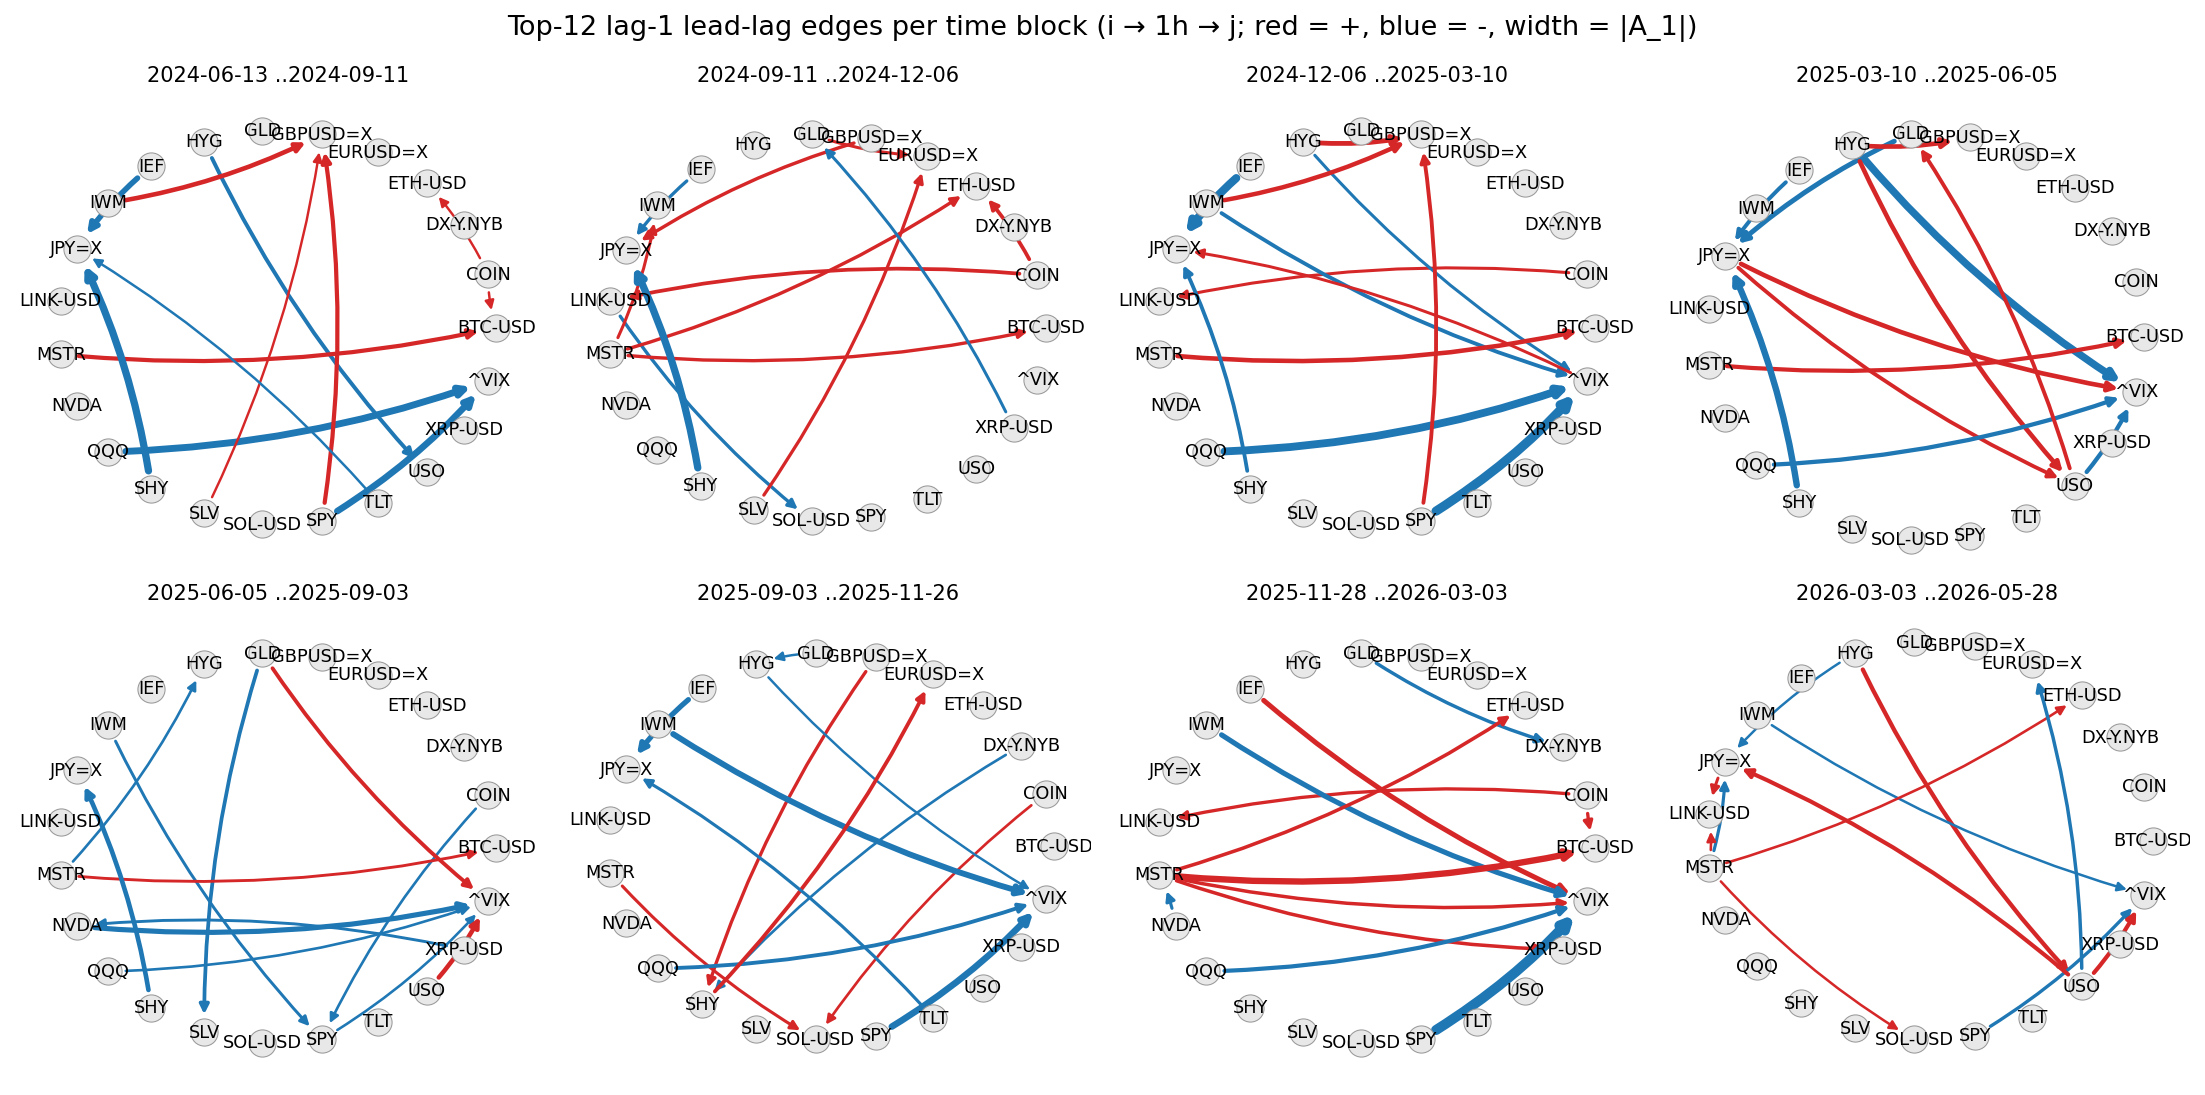
\includegraphics[width=\textwidth]{top_lag1_edges_per_block.png}
\caption{Top-12 lag-1 lead-lag edges per block ($i$ at $t{-}1$h $\to j$ at $t$;
$=|\A_1|$, $\sim 20\times$ weaker than $\W$, note the smaller weights). A few edges
recur: equities lead VIX down the next hour (SPY/QQQ/IWM$\to$VIX, negative), front-end
rates lead the yen (SHY/IEF$\to$JPY), and the RTH-traded crypto proxies lead spot crypto
(MSTR$\to$BTC in six of eight blocks, COIN$\to$LINK), most plausibly a liquidity/
session-timing effect rather than information flow. As with $\W$, this is persistent
lead-lag \emph{association}; with a temporal ordering it is closer to Granger precedence
than $\W$, but still not structural causality.}
\label{fig:lag1}
\end{figure}

\paragraph{Selection corroborates the null.}
Independently of the permutation tests, held-out-likelihood $(\lambda,\gamma)$
selection on the real panel drives the fusion penalty to $\gamma\to 0$ (held-out NLL is
minimized at $\gamma{=}0$; BIC selects a negligible $\gamma{=}0.02$, which alone shrinks
$\|\Wd\|_1$ by $\sim\!63\%$). Where the synthetic ground truth had selection choosing
$\gamma>0$ in every seed, the real data has selection finding \emph{no change graph
worth encoding}, an orthogonal witness to the same null.

\section{Discussion and limitations}

The methodological contribution is validated on ground truth: a fused, Student-$t$ DBN
with an exact-prox ADMM solver recovers a sparse change graph substantially better than
the DYNOTEARS-equivalent, with the advantage attributable primarily to the exact prox,
secondarily to the heavy-tailed loss and fusion, and robust to a distribution-free
transform and to principled penalty selection. The empirical study delivers a
carefully-controlled negative result: scheduled macro events raise volatility
(which the matched null absorbs) but do not measurably reorganize the conditional
dependency graph at hourly RTH frequency over this window, at global or edge-wise
resolution, for contemporaneous or lagged structure, and held-out selection
independently declines to encode a change graph.

Several limitations bound these conclusions. (1) Frequency and timing: real
cross-asset lead-lag plausibly lives at sub-hourly scales an hourly two-year panel
cannot resolve, and 08:30-ET releases are observed only post-open, so a minute-scale,
near-24h panel is the natural next test. (2) Event-regime size: with $104$ event
bars, fusion has little out-of-sample signal and exact support recovery is hard, which
is exactly why ground-truth simulation, not held-out density, is the right yardstick.
(3) Scope: the closed-form prox is $K{=}2$ only; $K>2$, learned $\nu$, and
per-regime scales are deferred. (4) Identifiability: with free per-variable
scales we make no equal-variance Gaussian identifiability claim
\citep{peters2014identifiability}; Student-$t$ here is a robust $M$-estimator yielding
more efficient recovery under heavy tails, as the synthetic results bear out.

\section{Conclusion}
We presented FR-tDBN, a fused-regime Student-$t$ dynamic Bayesian network whose
estimand is a sparse change graph, solved by consensus ADMM with a closed-form
fused-lasso prox inside the NOTEARS augmented-Lagrangian loop. On a
var-sortability-controlled benchmark it recovers the change graph far better than the
DYNOTEARS-equivalent, driven mainly by the exact-prox solver. Applied to a complete
cross-asset panel, it validates the contemporaneous heavy-tailed DAG but finds,
under volatility-matched nulls and corroborating model selection, that scheduled macro
events do not reorganize the dependency structure at hourly resolution: an honest,
controlled null distinct from the validated method.

\paragraph{Reproducibility.} All results come from one codebase (\texttt{frtdbn/});
the synthetic grid/sweep, real-panel run, robustness, baselines, selection, and figures
are produced by scripts in \texttt{scripts/}, with $100$ unit tests passing. Data is
hourly Yahoo Finance; the event calendar is verified against official BLS/Fed schedules.
All code and data are available at \url{https://github.com/0xknxwledge/TTIC31180FinalProject}.

\paragraph{Acknowledgments.} Drafting and figure code were assisted by Claude
(Anthropic) and cross-checked by Codex; all results, analysis, and final content are
the author's.

\bibliographystyle{plainnat}
\bibliography{references}

\end{document}
